% !TEX root = ../../thesis.tex

\cleartoleftpage
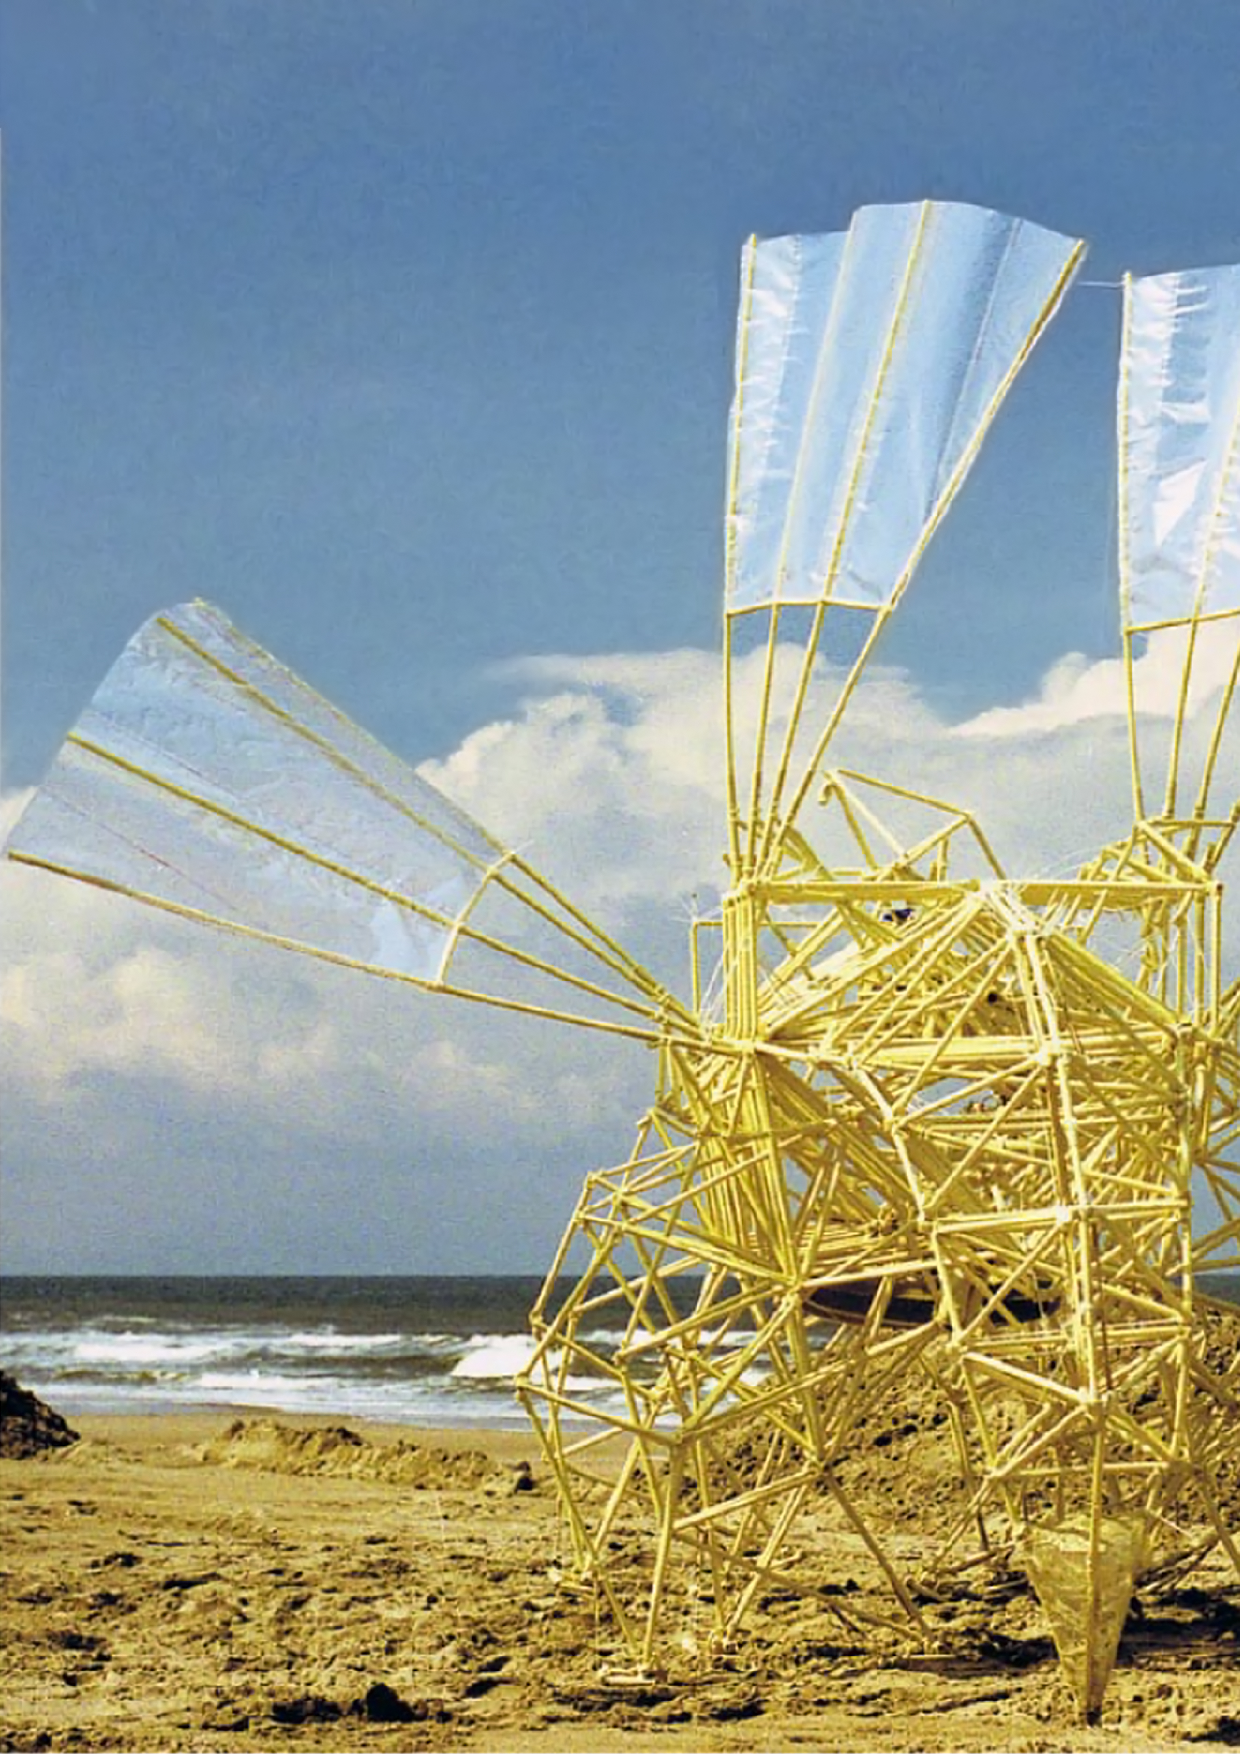
\includepdf{../media/chapter_illustration/jansen.pdf}

% Kant les hommes sont comme les oiseaux

\chapter{Exploring robotics morphology: some fascinating work} % (fold)

\cleanchapterquote{The cognition needs a body to think}{Rodney Brooks}

\section{Introduction} % (fold)

\begin{figure}[!b]
\centering
    \subfloat[][The turtle robot.]{\label{fig:walter_robot}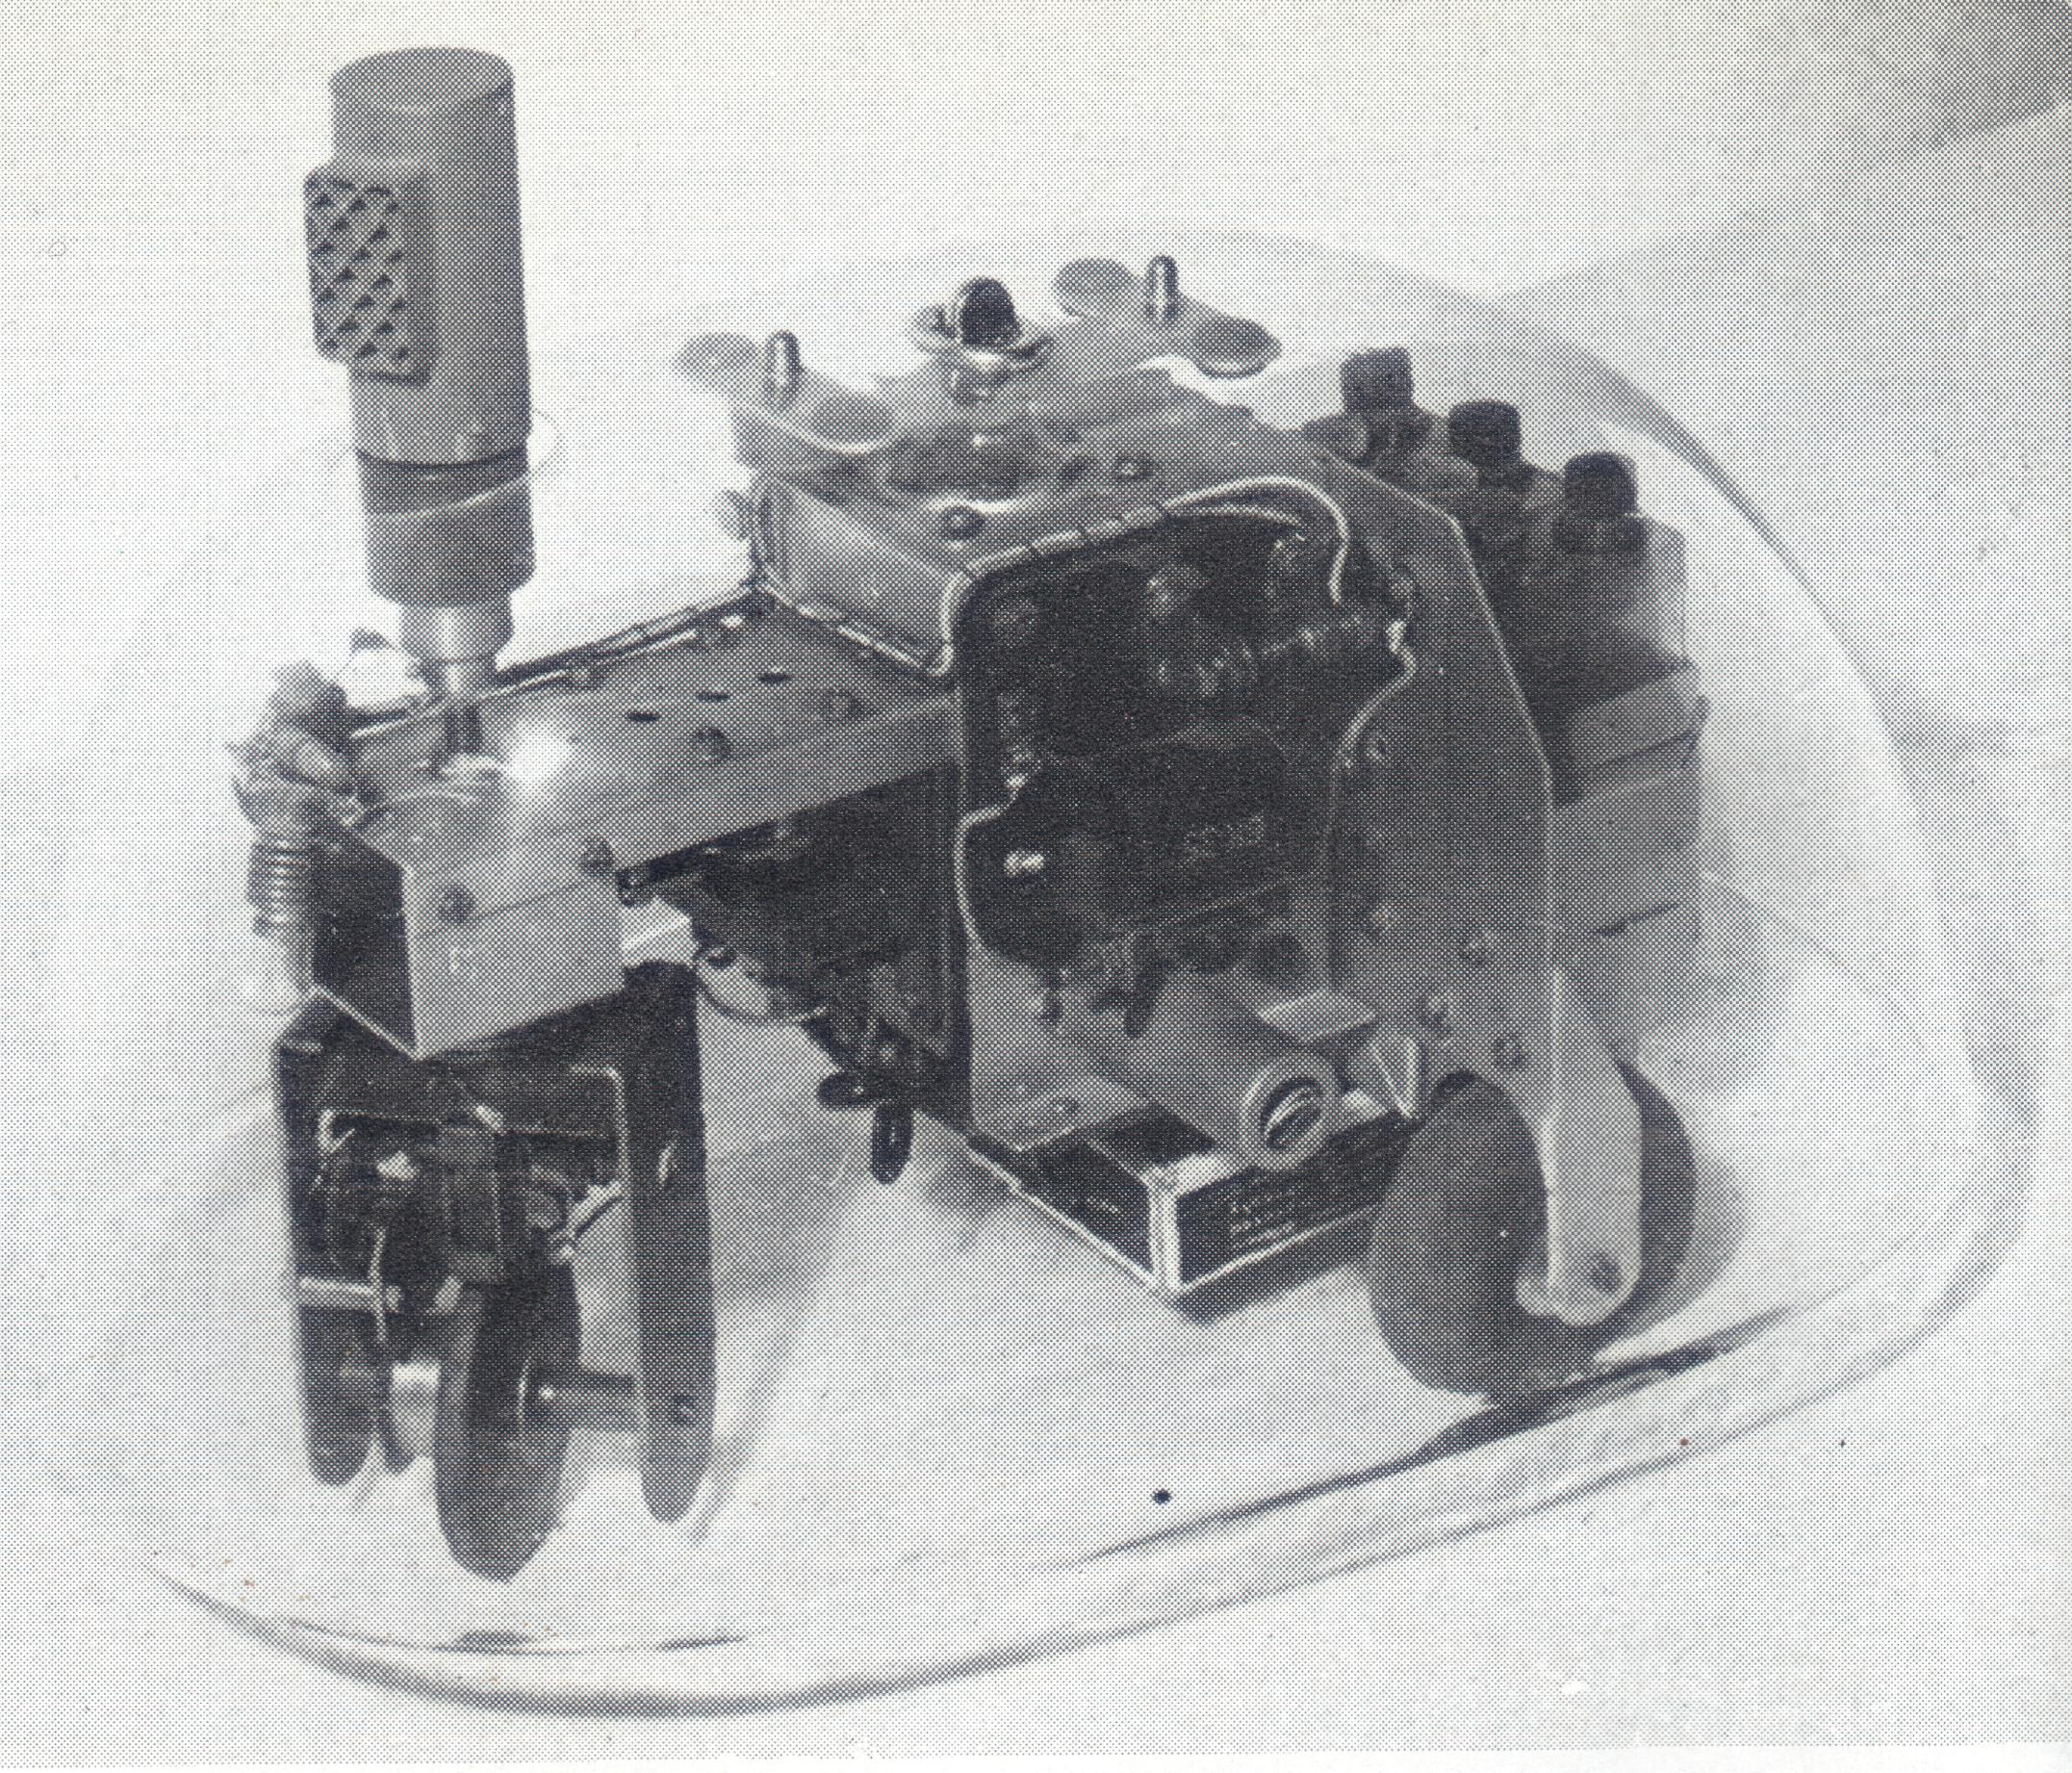
\includegraphics[height=6cm]{walter_turtoise_robot.jpg}}
    \hfil
    \subfloat[][Demonstration of obstacle avoidance behavior.]{\label{fig:turtle_behavior}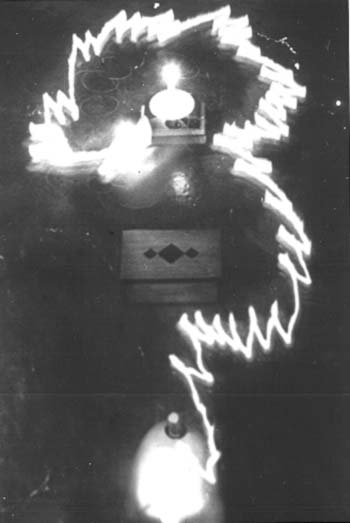
\includegraphics[height=6cm]{turtoise_behavior.jpg}}
    \caption{The W. Grey Walter's turtle was a really simple robot using direct analog connexion between light sensors and wheel actuator. The behavior of the robot was determined by the way sensors and actuators was plugged. It could demonstrate complex behavior such as obstacle avoidance or returning to its recharging station.}
    \label{fig:turtle_robot}
\end{figure}


\textbf{todo: y'a plein de robot, expliquer differement les turtles robots. \url{http://www.futura-sciences.com/magazines/high-tech/infos/dossiers/d/robotique-robotique-a-z-178/page/2/}}


In 1949, Elmer and Elsie, also known as turtle robots (see \figurename~\ref{fig:walter_robot}), created by the cybernetic pioneer W. Grey Walter, could be considered as one of the first robots in the robotics modern history era (1950-now). Back at this time, the transistor was just invented (1948)~\cite{brinkman1997history} and calculus was done with mechanical machines (see the focusbox). The turtle robot was entirely analogical but was able to demonstrate complex behaviors (see \figurename~\ref{fig:turtle_behavior}). Without any "reflexion" or internal representation of itself and the world, this robot, thanks to its conception and the direct analogical interaction between sensors and actuators was able to avoid obstacles and reach its charging station~\cite{walter1950imitation}.
These complex behaviors which can be compared with the ones found in nature were in fact done without any kind of intelligence and were actually emergent from the interaction between the robot morphology (i.e. where sensors are placed and how they are connected with actuators) and the robot environment (i.e. light sources).

\begin{figure}[]
    \centering
    \begin{boxedminipage}{0.95\textwidth}
        \textbf{Mechanical calculus}\\
        Once upon a time, in a age transistors were not here, complex calculus was done using mechanical properties.
        Using complex mechanisms the very first calculators were fully mechanical machines (see \figurename~\ref{fig:mechanical_computer}).

        The first freely programmable, binary, floating-point, general-purpose mechanical computer in the world was the Z1 constructed by Zuse between 1936 and 1938 (see \figurename~\ref{fig:zuse_z1}).
        This "computer" contained approximately 30,000 components and was incredibly sophisticated, making the Z1 suitable for a wide variety of engineering and scientific applications.
        Introduced by Curt Herzstark in 1948, the Curta (see \figurename~\ref{fig:curta_calculator}) is a small, hand-cranked digital mechanical calculator.
        It can be used to perform addition, subtraction, multiplication, division, and (with more difficulty) square roots and other operations.
        The Curta's design is a descendant of Gottfried Leibniz's Stepped Reckoner and Thomas's Arithmometer, accumulating values on cogs, which are added or complemented by a stepped drum mechanism.
        It has an extremely compact design: a small cylinder that fits in the palm of the hand.

        These two examples show that even pure calculus is achievable using only morphological properties (here mechanical) and was used during dozens of years for scientific applications.


        Curtas were considered the best portable calculators available until they were displaced by electronic calculators in the 1970s.

        \begin{center}

            \subfloat[][Zuse Z1 (1936)]{\label{fig:zuse_z1}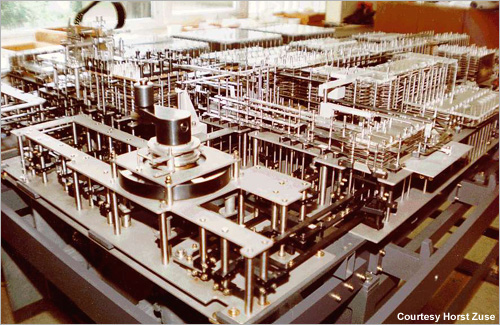
\includegraphics[width=0.42\linewidth]{hist-z1-reconstruct.jpg}}
            \hfil
            \subfloat[][Curta]{\label{fig:curta_calculator}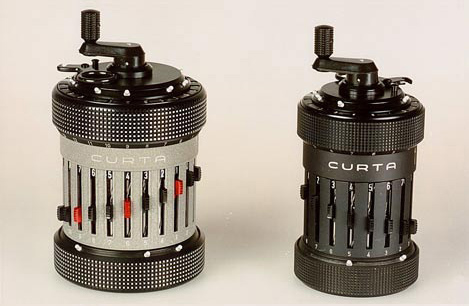
\includegraphics[width=0.42\linewidth]{curta_calculator.jpg}}
            \caption{Mechanical calculus machines}
            \label{fig:mechanical_computer}

        \end{center}

    \end{boxedminipage}
\end{figure}


\subsection{The cognitivist approach limits} % (fold)


With the arrival of numeric computers, researchers imagined the opening of a field where it could be possible to replace pre-wired analogical electronic behaviors by the use of computer running programs. Not dependent on the hardware platform, robots would be therefore more versatile.
The artificial intelligence (AI) term was introduced in a workshop organized in 1956 by a MIT professor John McCarthy (REF). Globally participant were convinced, that by using the notion of computation or abstract symbol manipulation, it would be possible to reproduce interesting abilities similar to human ones~\cite{kaufmann1979machines}~\cite{haugeland1989artificial}. The symbol-processing paradigm or cognitivistic paradigm see the cognition as pure computation. In other word, the actual intelligence process is the abstract algorithm or the program doing calculus. Eventually, researchers following this paradigm no longer saw the physical incarnation as a relevant component. Cognitive and computationalists hypotheses stating that the thought is reducible to a set of symbolic calculations are being established~\cite{fodor1987psychosemantics}. The body, for its part, is forgotten, irreparably separated from the mechanisms of intelligence~\cite{kaplan2008corps}.
In addition, the robot body became a handicap which often ruins the efficiency of algorithms and programs created by AI researchers. Indeed, the real world body is non perfect, there is some noise on sensors acquisition, there is gravity, friction and inertia acting on actuators, and the environment is always changing and unpredictable.

To overcome these issues of real world applications, the other side of the robotics community, still interested in the hardware challenges strives to design more reliable and powerful robots which can react as fast and as close as possible to the model used for its control. To do that, it is needed to have way more precise sensors and powerful enough actuators to overcome inertia and mechanical friction. Thanks to these work on hardware, industrial robots became more and more fast and precise, enough to outclass any human on specific assembly tasks.

However, even with really efficient robots, artificial intelligence failed to show results comparable with the expectations researchers and society had. Robots are able to solve incredibly complex task such as chess game or able to achieve highly precise tasks in manufacture but require perfectly controlled and predictable environment. Going outside this known environment seems impossible to program and none of them is able to act fluently in the real world.


\textcolor{TODO}{But unlike virtual worlds, the real world is challenging in various ways. It is not possible to enable omniscience: we have not access to the knowledge of the whole world state and parameter, the measures a robot can take are limited, take time and are noisy while the action took are always different that. Finally, the world state is never clearly defined, based on precise discrete states;~\cite{piefer06}.
Unlike virtual workds, the real-world challenges an agent in various ways. First, because real-world agents are emboied, acquisition of information always take time. Second information thatn an agent can acquire about real world is always very limited. We can never have complete information. This situation is different from a formal game like chess, where knowledge of the board positon constitutes all the information about the state of the game. Third information acquired trhough them will always contain errors. Fourth the real world s not characterized by clearly defined, discrete  states, the weather is never simply goof or bad.
The real wolrd has its own dynamics -things out in the world happen even if not do anything- ther is always time presure due to ongoing change. Thus agent are always forced to act whether they want to or not.
Related to this point, the real world is a highly complex dynamical system, making it intrinsically unpredictable because of its nonlinear nature and its sensivity to initial conditions (hebert Simon has coined the term bounded rationality to designate, in essence, decisions that have to be taken under such circumstances (Simon, 1976,1969e)).}

Thus classical approach known great successes to solve abstract problems such as chess game, search engine, text processing, however it failed in the understanding of natural forms of intelligence which requires a direct interaction with the real world. This is especially the case when we think in the current state of the art for interaction with human (natural language) or object (grasping) and the locomotion in an open environment (walk, run, ride a bicycle).

\subsection{Emergence of the embodiment paradigm} % (fold)

Stuck with these major issues raised by acting in the real world, a kind of crisis of the artificial intelligence happened in the 1980's and the cognitivist paradigm was questioned. While some researchers of the field introduced new tools such as neuronal networks, another part questioned the "cognition is computation" approach and the irrelevance of the body.
Thanks to researchers such as Rodney Brooks~\cite{brooks1986achieving}, Rolf Pfeifer~\cite{pfeifer2001understanding} or Luc Steels~\cite{steels1995artificial}, a novel paradigm emerge: the cognition needs a body to think. The embodied artificial intelligence rejects the symbolic approach and postulates that it is not possible to have intelligence without the body and the environment~\cite{pfeifer2001understanding}. Rather than postulating there is a hierarchical structure in which the brain control the body, the new theory focuses on the interaction between the two systems, even for mathematical thinking we could assume is purely abstract~\cite{lakoff2000mathematics}.

Following this paradigm, several researchers tried to tackle challenges in which the classical cognitivist approach failed i.e. the understanding of natural forms of intelligence which requires a direct interaction with the real world. The locomotion is a great example of task where the classical robotic approaches did not get expected results.

Animals are incredibly skilled. Even if we consider insect with a brain thousand of times smaller than the human one, theirs abilities to move in an open world is just incomparable with the most advanced current robots. One important reasons for this is that in the classical view, the ability to figure out where you are is based in detailed inner models or representations either have to be programmed into the robots or learn by interacting with the environment and continuously updated. The more complex these models are, the more effort is needed to acquire the relevant data to maintain them leading to major problem when learning task in a highly dimensional spaces (plein de REF). Brooks even argued that intelligence always requires a body and that we should forget about complex internal representations and models of the outside world; that we should not focus on sophisticated reasoning processes but rather capitalizer on the system-environment interaction~\cite{brooks1991intelligence}~\cite{brooks1995intelligence}. Then he started to work on the insect locomotion because if we understand the insect-level-intelligence it will be much easier and faster to understand and build human-level intelligence~\cite{brooks1996prospects}.

\textbf{TODO: petite review du boulot de brooks avec les insects}

Exploring the role of the morphology and how it shapes the ways we think appears a fascinating open field. Indeed, exploring the interaction between body properties and cognition could lead to both a better understanding of animal's behaviors (human being in particular) and to build robot more adapted and robust to an open environment with unpredictable interaction.

Thus an interesting evolution of the last decades is the demonstration of the importance of the morphology for sensorimotor control, cognition and development. The researches community exploring the embodiment paradigm has grown but surprisingly not as much we could imagine with classical paradigm fails. However, new work arises introducing new principles we will describe in this chapter such as morphological computation, compliance or ecological balance, emergence.

In the context of this thesis we will talk about intelligence with the meaning, ability to move in a natural environment and interact with people and objects.



\section{Exploring the role of robot morphology} % (fold)


The achievement of robust locomotion in a natural environment is one of the major current challenge for robotics researchers. For decades and it is still mostly the case, the challenge of locomotion for robotic agent was only tackles through symbolic abstract and complex computation of internal model and representation of the world. The body is reduced to a noisy interface between the abstract algorithm and the real world.
However, regarding the nature, it appears obvious that an animal morphology deeply change the way it can act in its ecological system and so it has evolved trying to optimize its body properties.

For some reasons, in the robotics and artificial intelligence field the link between the body properties and the ability for a robot to move in an ecological environment does not seems as obvious. The fact that the ability to act and achieve complex task are due to the brain computation is so deeply grounded that it event affects the general public.

However, while we can think there are indeed calculus necessary to achieve complex tasks, there is no reason it should be explicit with a precise internal models or representations of the physical world while it could be directly done through body properties.

Therefore since the 80's, considering the robot morphology defined as \emph{any characteristic which defines the physical structure of the robot such as link sizes, number of links, joint characteristics, mass distribution, actuator characteristics, material properties, sensor characteristics and sensor placements}~\cite{paul2006morphological}, novel research topics appeared exploring the role of robot body morphology towards the achievement of complex tasks in natural world, especially robot locomotion.


\subsection{Morphological computation principle} % (fold)

Introduced by Rolf Pfeifer~\cite{pfeifer2005morphological}, the morphological computation principle states that a part of the computation needed in the achievement of a given task can be done implicitly through the interaction of physical form with the ecological niche environment.

\textcolor{TODO}{The fact that the morphology of a robot affects its control requirements has become increasingly evident in robotics. Not only does the morphology determine the behaviors that can be performed, but also the amount of control required for these behaviors. Particularly in systems where behavior is obtained through purely sensory-motor interactions of the body with the environment, the morphology is of prime importance. Nonetheless, even in other robotic systems, a relationship has been found to exist between morphology and control requirements, in that some morphologies yield themselves to being more easily controlled than others.
This relationship was first observed and characterized by Pfeifer as the morphology and control trade-off ~\cite{pfeifer2001understanding}, but the mechanisms underlying this relationship have been unclear. The fact that simple physical interactions give rise to computation indicates the theoretical possibility for the dynamics of the morphology to play a computational role in the system, and thereby to subsume part of the role of control~\cite{paulinvestigation}.}


\subsection{Passive and semi-passive walking} % (fold)

The role of morphology in robot biped locomotion has been particularly explored through the research on passive dynamic walkers~\cite{wisse2007passive}.

Bipeds walking on slightly inclined plane appeared as toys in the early twentieth century. Their legs are straight and they rock on sides to allow feet lift off the ground. The analysis of the behavior of such systems, purely passive, is much more recent. Indeed, an advantage of such object is their low energy consumption. The energy supplied to the system comes from the variation of potential energy due to the slope. It compensates the lost energy during impact.

The unipodal transfer movement is similar to a passive pendulum and arises from the correct combination of an initial pulse and coupled gravity-inertial effects. The behavior of the walker is then to the inverted pendulum.

In the early 90's, Tad McGeer, coming from an aeronautic background, formalizes the idea of a compass biped with free articulation by the concept of synthetic wheel~\cite{mcgeer1990passive}.
The dynamics of the system is formalized by an equation of motion linearized close to an average vertical position of the legs and an equation of shock upon contact foot/ground modeling energy dissipation~\cite{mcgeer1992principles}.

\begin{figure}[h]
\centering
    \subfloat[][]{\label{fig:}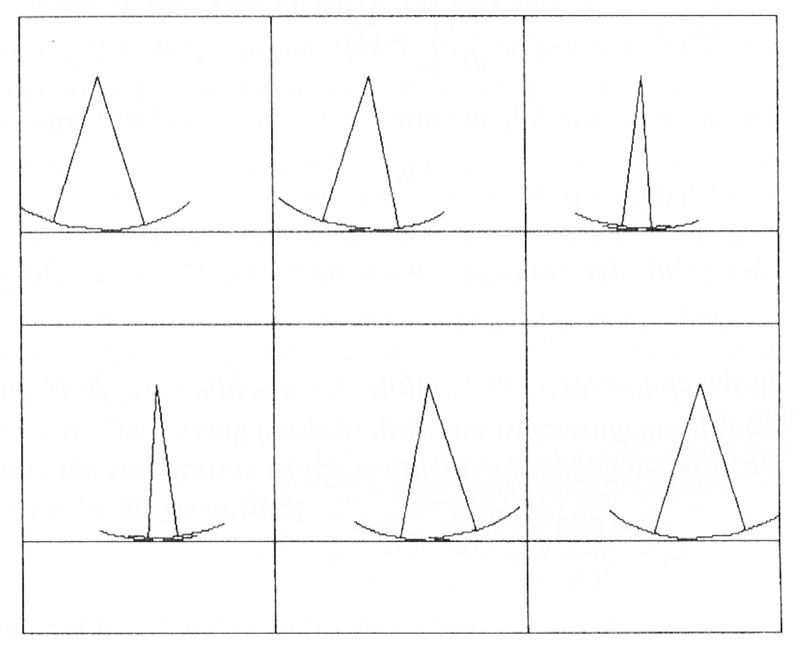
\includegraphics[width=0.4\linewidth]{simple_leg_wheel.jpg}}
    \hfil
    \subfloat[][]{\label{fig:}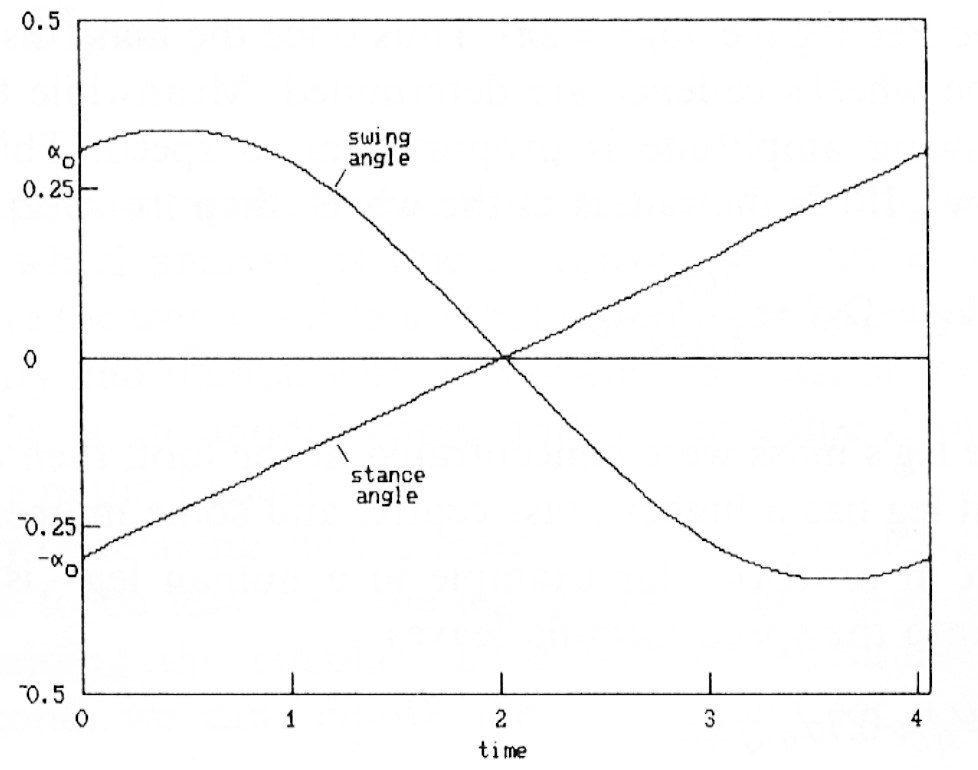
\includegraphics[width=0.4\linewidth]{simple_leg_wheel_trajectories.jpg}}
    \caption{The simplest of walking models is the synthetic wheel, a biped with straight legs and semicircular feet (a). The stance leg rolls forward steadily like a spoke in a wheel, while the free leg swings ahead like a pendulum. Support is transferred between legs when their speeds and angles match (b). The cycle is naturally stable and will repeat continuously, thus synthesizing the motion of ordinary wheel~\cite{mcgeer1992principles}.}
    \label{fig:synthetic-wheel}
\end{figure}


The tuning of initial conditions conducting to a passive movement is performed numerically, after a step, the robot should be back to its initial state. This model allows to obtain a robot cyclic walking gait completely passive (without motorization) and stable on an plan, slightly inclined by a few degrees. The potential energy gained during the descent exactly compensates energy dissipated during impacts.


\subsubsection{Passive walkers} % (fold)

\begin{figure}[]
\centering
    \subfloat[][Tad McGeer with his prototypes]{\label{fig:tad_mcgeer}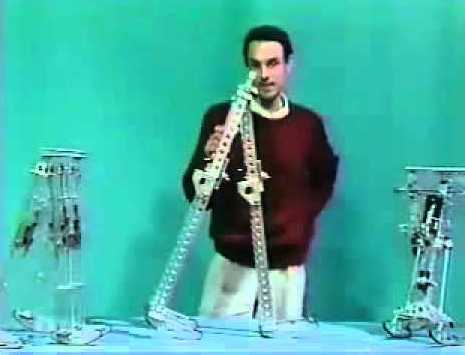
\includegraphics[width=0.49\linewidth]{tad_mcgeer.jpg}}
    \hfil
    \subfloat[][Passive walker robot]{\label{fig:mcgeer_walker}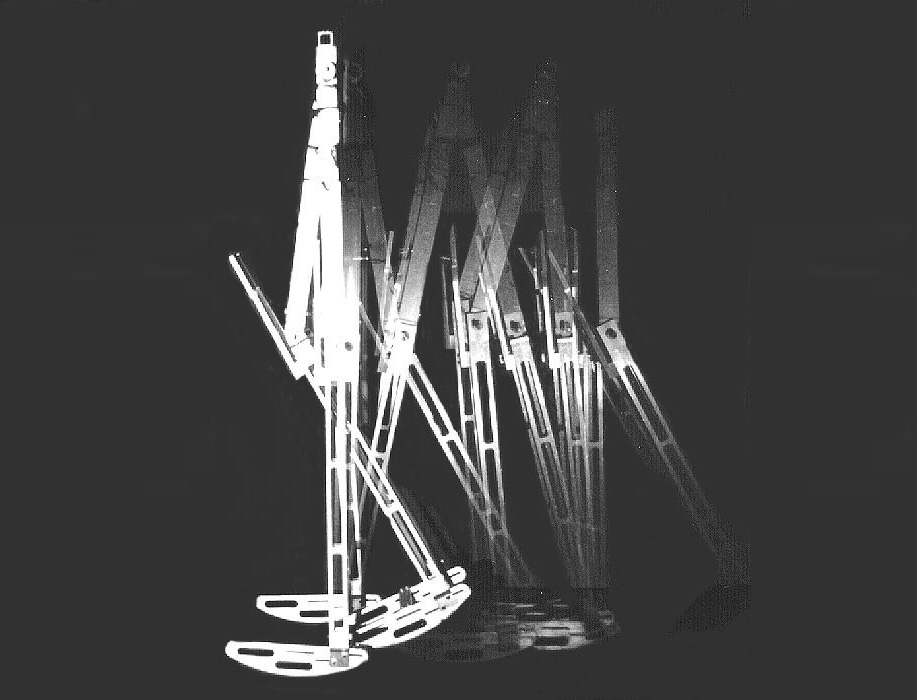
\includegraphics[width=0.49\linewidth]{mcgeer_walker.jpg}}
    \caption{}
    \label{fig:mcgeer_work}
\end{figure}

Tad McGeer has also showed that passive walking can be obtained on a bi-articulated robot~\cite{mcgeer1992principles}. An appropriate feet shape and a judicious mass distribution allow the generated footstep combining a forward pendular swinging movement on its stance leg and a swing with spontaneous flexion of the leg transferred. To make this motion possible, a device must prevent against leg bending during the stance phase.
The dynamic behavior is mainly determined by three dimensionless parameters: the length ratio, the mass ratio and the slope of the planar support ~\cite{Garcia1998}.


\subsection{Semi-passive walkers} % (fold)
Passive robots are limited to walking on inclined ground, they can not have a passive trunk and finally they are locally stable robots, the limit-cycle attraction domain is small.

Thus this work has been pursued with the apparition of semi-passive walkers combining both specific passive properties and low power actuation to increase their robustness~\cite{Anderson2005}. We can note the work of Collins~\cite{collins2005bipedal} which explored the case of semi-passive 3D biped robot. Its morphology is based on particular mass distribution, knee locking, round feet and springs on the legs to generate an efficient walking gait while keeping its lateral and frontal balance. The concept of 3D semi-passive robot has been pushed even further with the realization of a complete humanoid robot with trunk, arms and head: the robot Denise~\cite{wisse2005three} and Flame presented in~\cite{Hobbelen2008}.

\begin{figure}[]
    \begin{center}
        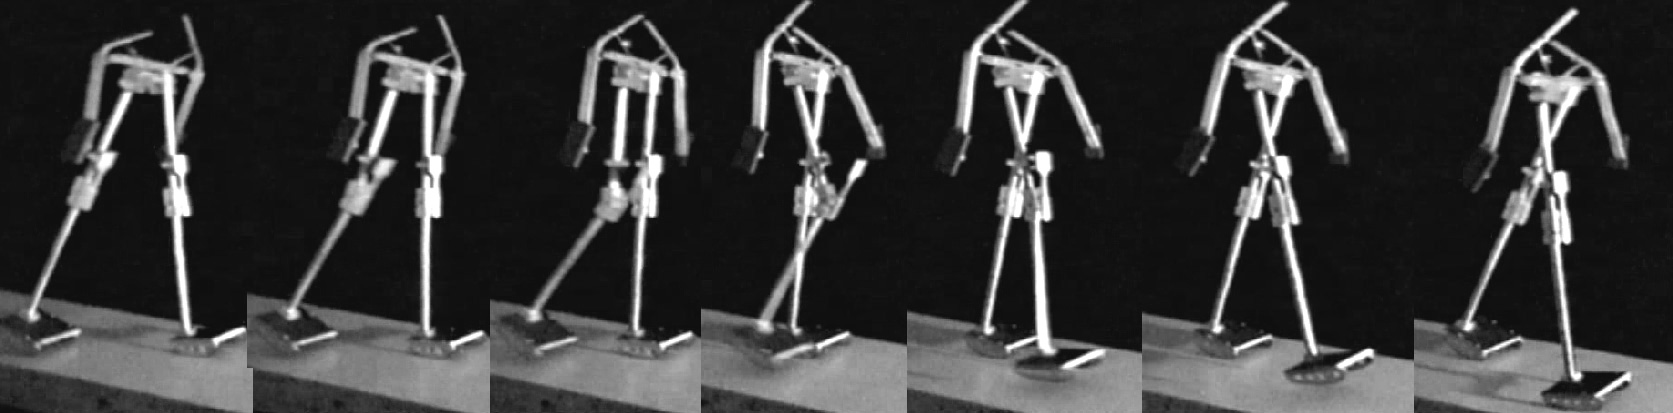
\includegraphics[width=0.99\linewidth]{cornell_biped_series.jpg}
    \end{center}
    \caption{Caption here}
    \label{fig:figure1}
\end{figure}

\begin{figure}[]
    \begin{center}
        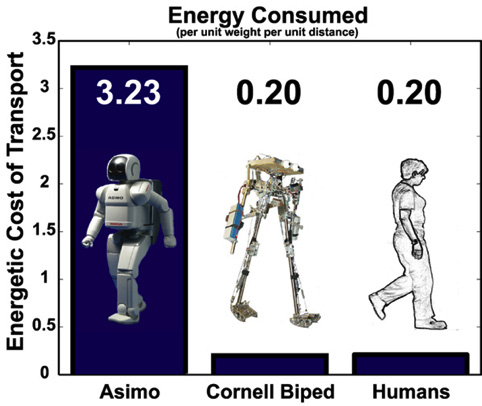
\includegraphics[width=0.6\linewidth]{comparison_cost_transport.jpg}
    \end{center}
    \caption{Caption here}
    \label{fig:figure1}
\end{figure}


\subsection{Emergence of complex behaviors} % (fold)

Finding the rules that can lead to a desired behavior is more difficult than explaining an actual complex behavior when we can observe an agent interacting with its environment. Because the fact that the behavior itself cannot be preprogrammed but is always the result of an agent-environment interaction, we must design for emergence rather than directly for a specific behavior~\cite{Pfeifer06}. It is called the design of emergence~\cite{Steels1991emergence} which remains an open question how this can be done systematically. At the moment, design for emergence is rather an art than a hard-core engineering discipline.

It is precisely in the art field that we find one of the most fascinating examples. Theo Jansen is a kinematic sculptor. This artist playing with field frontiers, between engineering, research and art is the designer of the sand beasts (see \figurename~\ref{fig:theo_jansen_beast}).

\begin{figure}[]
    \begin{center}
        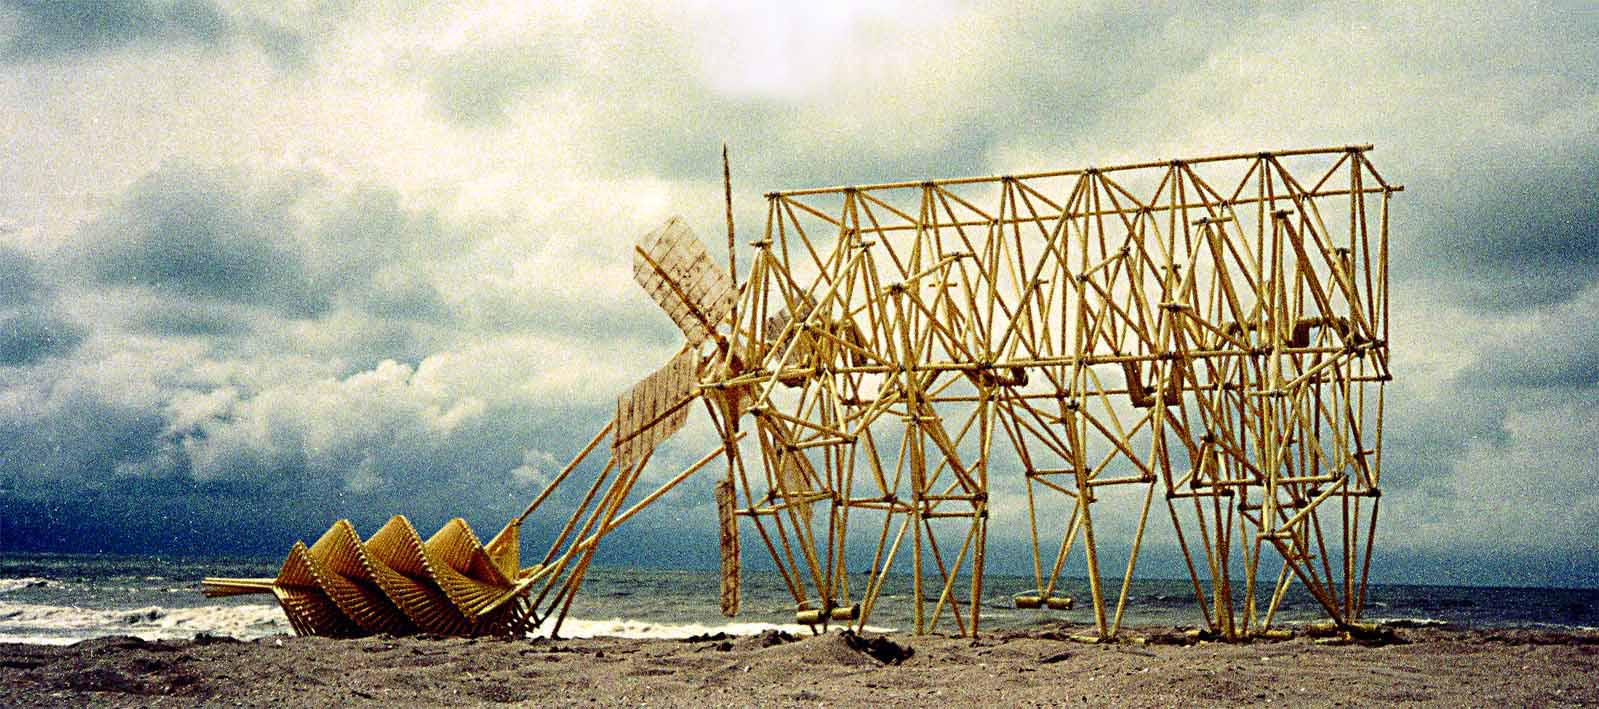
\includegraphics[width=0.99\linewidth]{theo_jansen_beast.jpg}
    \end{center}
    \caption{Caption here}
    \label{fig:theo_jansen_beast}
\end{figure}

These giant structures move using a really clever mechanisms composed of eleven rods which lengths have been tuned by numerical optimization. This system produces a walking motion(see \figurename~\ref{fig:beast_mechanism}) with a center of rotation always remaining at the same level, for this reason Theo Jansen likes to say he "reinvented the wheel" but adapted to the environmental niche of his creatures .i.e. the beach.

Since the beginning of this work, Theo Jansen created dozens of creatures, being more and more evolved. However, the very basic mechanism remains the same, both simple because it is composed by only one degree of freedom, and complex because the length ratio between the eleven rods are critical and must be equal to specific numbers. Thus, using only really basic material, electric plastic tubes, Theo Jansen created multi-legged creatures capable of moving in the sand, powered by the wind~\cite{jansen2007theo}.


\begin{figure}[]
\centering
    \subfloat[][]{\label{}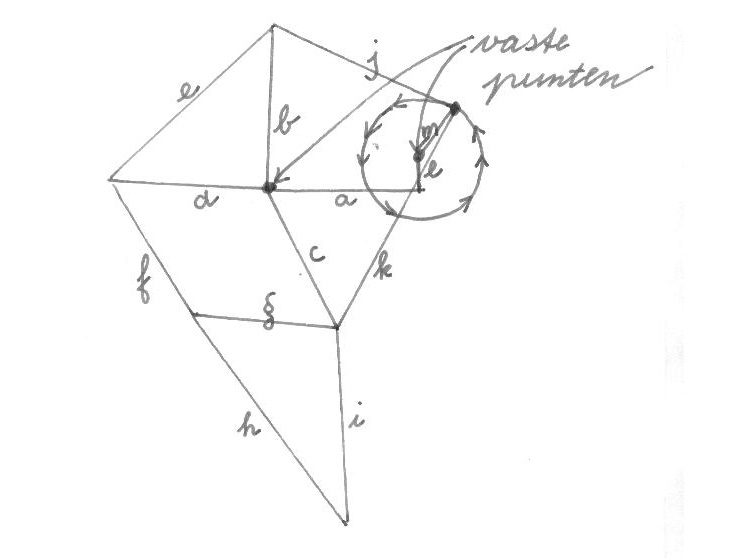
\includegraphics[width=0.32\linewidth]{strandbeest_theory.jpg}}
    \hfil
    \subfloat[][]{\label{}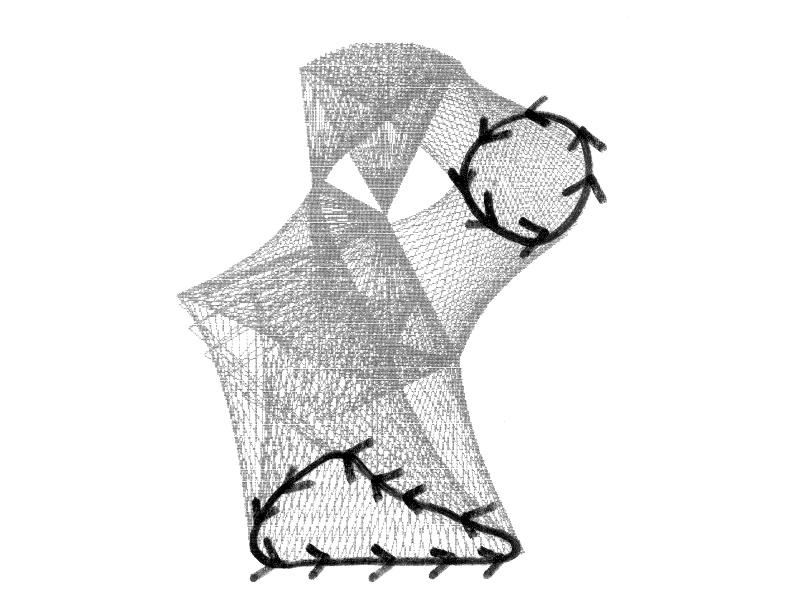
\includegraphics[width=0.32\linewidth]{strandbeest_motion.jpg}}
    \hfil
    \subfloat[][]{\label{}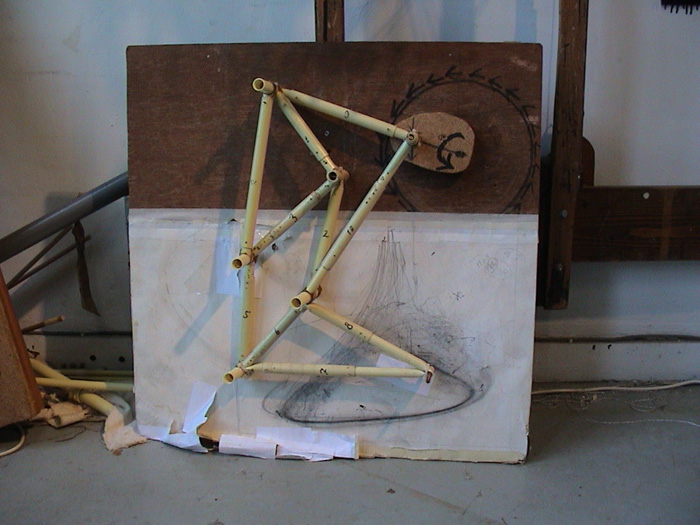
\includegraphics[width=0.32\linewidth]{strandbeest_leg_element.jpg}}
    \caption{}
    \label{fig:beast_mechanism}
\end{figure}



Evolution of his work, conducted to several improvements. In this video: \url{http://youtu.be/rWbU3eV4ZpQ}, 72 legs moving at the same time using one cranks. But he also extended the mechanism to add a kind of independence. For instance, he added lemonade bottles to store energy. These bottle are used as pressure tank fulled using pumps powered by the wind. Beasts can use this stored energy in case the wind fade away.

Also, a natural enemy of these beasts is the sea, using the same basic material, Theo Jansen created sensors able to detect the water and reverse the way beast move. The same principle allows also these beast to avoid obstacle.

Thus the work of Theo Jansen goes beyond the kinematic art and is really instructive for the robotic and IA research fields. Indeed, thanks to a specific morphology adapted to their environmental niche, his creatures are able to act autonomously and "survive" in the real world. No computation, no abstraction, the appeared intelligence of these creatures only came from a direct interaction between their particular morphologies and the environment. Based on low cost materials, yet clever mechanisms, his work is a meaningful proof of concept showing how the morphology of an agent can lead to the creation of complex behavior such as ones could called them "intelligent".

\section{Conclusion} % (fold)

